\chapter{Các công nghệ sử dụng}
\section{Xây dựng tính năng autoscaling với custom metrics}

\subsection{Định nghĩa}
\noindent Theo Google Cloud Platform\footnote{Dựa theo link: https://cloud.google.com/kubernetes-engine/docs/concepts/custom-and-external-metrics}, một \textit{custom metric} sẽ được truyền từ ứng dụng của bạn mà đang chạy trên Kubernetes.
\subsection{Đặt vấn đề}
\noindent Việc scale theo CPU và memory không hiệu quả với rest api.\\
\noindent Mặc dù các số liệu mặc định do Kubernetes cung cấp, chẳng hạn như mức sử dụng CPU và bộ nhớ dựa trên yêu cầu tài nguyên, rất hữu ích trong nhiều tình huống nhưng chúng có thể không đủ cho tất cả các ứng dụng. Mở rộng quy mô dựa trên giới hạn tài nguyên đảm bảo rằng ứng dụng của chúng ta có thể xử lý các khối lượng công việc khác nhau mà không đạt đến mức tài nguyên tối đa được phép. Số liệu tùy chỉnh cho phép chúng ta điều chỉnh hành vi mở rộng quy mô của HPA dựa trên nhu cầu cụ thể của ứng dụng, cho phép tự động điều chỉnh quy mô chính xác và hiệu quả hơn.
\subsection{Cơ sở lý thuyết}
\textit{Nội dung tiểu mục được tham khảo từ chung một nguồn}\footnote{https://learnk8s.io/autoscaling-apps-kubernetes}\\[0.5cm]
% \noindent Nói về việc prometheus dùng để thu thập và cung cấp api server cho external metrics. KEDA cung cấp ScaledObject, được build dựa trên HPA để phục vụ cho việc scale dựa trên các metric thu thập từ prometheus.\\
% \noindent Có thể để các tóm tắt bài viết vào đây.
Khi xác định tài nguyên cho Horizontal Pod Autoscaler, chúng ta cần phải xác định metric mà ta cần theo dõi.

% Nhưng làm cách nào Bộ chia tỷ lệ tự động của Horizontal Pod biết cách lấy được các số liệu này?

Horizontal Pod Autoscaler truy vấn các metrics này từ Metrics Registry.
\begin{figure}[H]
  \begin{center}
    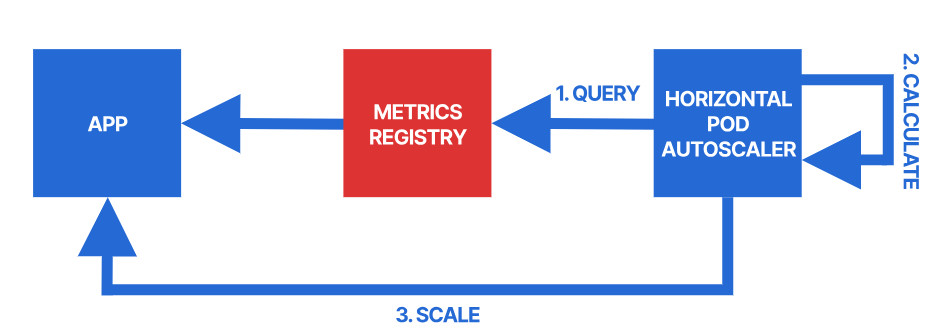
\includegraphics[scale=0.65]{images/phat/metrics_registry.jpg}
    \caption{Horizontal Pod Autoscaler queries flow}
  \end{center}
\end{figure}
Metrics Registry là vị trí trung tâm trong cluster nơi các metrics (dưới bất kỳ hình thức nào) được hiển thị cho clients (Horizontal Pod Autoscaler là một trong những ứng dụng clients này).

Mục đích Metrics Registry là cung cấp giao diện chuẩn cho client truy vấn các metrics.

Interface của Metrics Registry bao gồm 03 API riêng biệt:
\begin{itemize}
    \item The Resource Metrics API
    \item The Custom Metrics API
    \item The External Metrics API
\end{itemize}
\begin{figure}[H]
  \begin{center}
    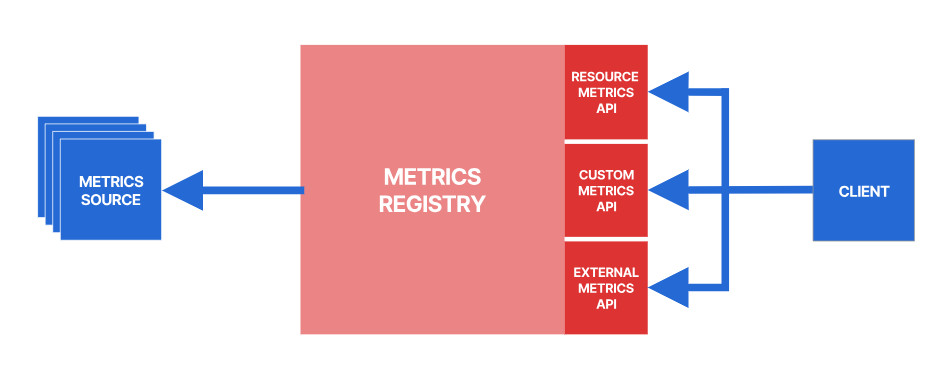
\includegraphics[scale=0.75]{images/phat/metrics_registry_API.jpg}
    \caption{Metrics Registry Interfaces}
  \end{center}
\end{figure}
Các API này được thiết kế để phục vụ các loại metrics khác nhau:
\begin{itemize}
    \item Resource Metrics API: số liệu sử dụng tài nguyên được xác định trước (CPU và bộ nhớ) của Pod và Node.
    \item Custom Metrics API: số liệu tùy chỉnh được liên kết với đối tượng nằm bên trong Kubernetes cluster.
    \item External Metrics API: số liệu tùy chỉnh được liên kết với đối tượng nằm bên ngoài Kubernetes cluster.
\end{itemize}
Vì vậy, để autoscale cho một ứng dụng, nhiệm vụ của chúng ta không chỉ là xác định cấu hình Horizontal Pod Autoscaler mà cũng phải hiển thị metrics mong muốn của mình thông qua Metric Registry.\\[0.5cm]
Đối với mỗi Metric API, chúng ta cần có Metric API Server tương ứng và chúng ta cần định cấu hình cho nó để hiển thị một metric cụ thể thông qua Metric API.\\[0.5cm]
Hơn nữa, chúng ta cần một Metrics Collector để thu thập các metrics mong muốn từ các nguồn (ví dụ: từ Pod của ứng dụng) và cung cấp chúng cho Metric API Server.
\begin{figure}[H]
  \begin{center}
    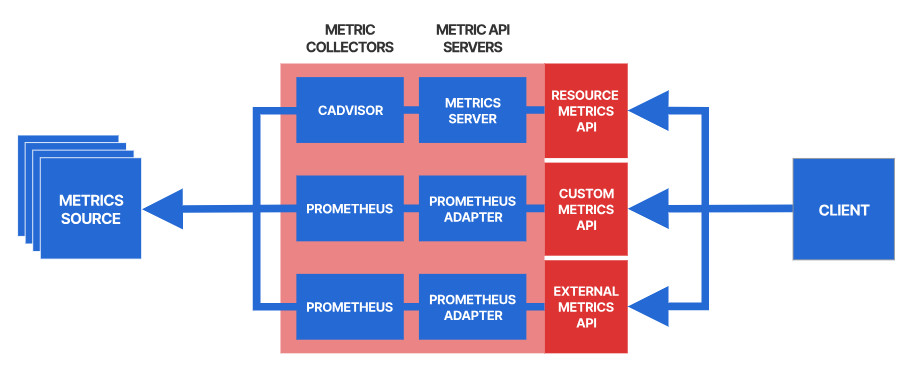
\includegraphics[scale=0.80]{images/phat/metric_registry_detail.jpg}
    \caption{Metrics Registry components}
  \end{center}
\end{figure}
Vì vậy, để expose metric thông qua một trong các API Metrics, chúng ta phải thực hiện các bước sau:
\begin{itemize}
    \item Cài đặt Metrics Collector (ví dụ: Prometheus) và định cấu hình nó để thu thập metric mong muốn (ví dụ: từ Pod của ứng dụng của bạn).
    \item Cài đặt Metric API Server (ví dụ: Prometheus Adapter) và định cấu hình nó để hiển thị từ Metrics collector thông qua Metrics API tương ứng.
\end{itemize}
$\ast$ \textbf{KEDA} sẽ hoạt động với vai trò như một Metric API Server, dùng để biên dịch các metric nhận được từ external server về các dạng dữ liệu mà HPA có thể hiểu được để tiến hành scale thông qua HPA. Như vậy khi sử dụng KEDA thì chúng ta sẽ không cần phải sử dụng Metrics Server từ K8s. Với KEDA chúng ta có 1 khái niệm là \textit{ScaledObject}, khi tạo ScaleObject nó là một phiên bản mở rộng của HPA để thực hiện việc scale pod.
\subsection{Công nghệ}
\subsubsection{Prometheus}
% TODO: Các phần này cần tự tìm thêm các nguồn khác để tìm hiểu
\textbf{a. Định nghĩa \footnote{https://www.tigera.io/learn/guides/prometheus-monitoring/prometheus-kubernetes}}\\[0.5cm]
Prometheus là một dịch vụ theo dõi và cảnh báo về hệ thống. Prometheus rất thích hợp với những hệ thống Microservices và có các dịch vụ Listening. Một hệ thống theo dõi chủ động như Prometheus sẽ giúp người quản trị phát hiện sớm những dấu hiệu cảnh báo xấu.\\[0.5cm]
Đối với những công việc liên quan đến Queue Job, mối nguy cơ luồng xử lý bị loop hoặc stop rất lớn. Lý do có thể đến từ tài nguyên phần cứng hoặc phần mềm được cài đặt không chính xác. Khi đó việc xem log của dịch vụ đó rất khó hoặc phụ thuộc vào may mắn. Với Prometheus các thông tin luôn được cập nhật và khi xảy ra lỗi, chúng ta vẫn có thể xem lại dữ liệu theo dõi một cách dễ dàng qua API của Prometheus.\\[0.5cm]
\textbf{b. Kiến trúc Prometheus \footnote{https://www.devopsschool.com/blog/what-is-prometheus-and-how-it-works}}

\begin{figure}[H]
  \begin{center}
    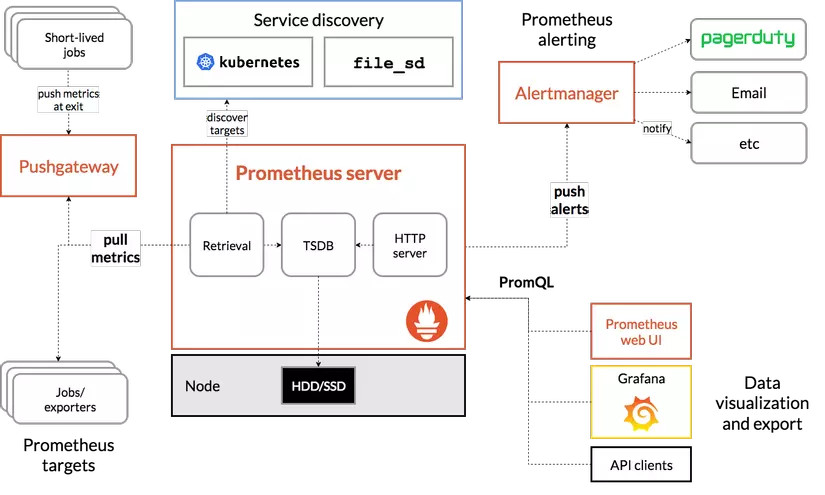
\includegraphics[scale=0.45]{images/phat/prometheus_architecture.jpg}
    \caption{Kiến trúc Prometheus}
  \end{center}
\end{figure}
\textbf{Các thành phần của hệ thống}\\[0.5cm]
\indent Có thể chia kiến trúc Prometheus thành 03 thành phần chính sau: 
\begin{enumerate}
    \item Prometheus Server
    \item Alert Manager
    \item Grafana
\end{enumerate}
\indent Cụ thể các thành phần chi tiết như sau:
\begin{itemize}
    \item \textbf{Prometheus Server}: thành phần chính thu thập, xử lý và lưu trữ dữ liệu chuỗi thời gian (time-series data).
    Nó chủ động liên tục lấy dữ liệu từ các điểm cuối (endpoints) của các dịch vụ và ứng dụng để thu thập thông tin về các metrics.
    Dữ liệu thu thập được được lưu trữ tại máy chủ Prometheus.
    \item \textbf{Push Gateway Prometheus}: sử dụng để hỗ trợ các job có thời gian thực hiện ngắn (tạm thời). Đơn giản là các tác vụ công việc này không tồn tại đủ lâu để Prometheus chủ động lấy dữ liệu. Vì vậy mà các dữ liệu chỉ số (metrics) sẽ được đẩy về Push Gateway rồi đẩy về Prometheus Server.
    \item \textbf{Jobs/Exporters}: hỗ trợ giám sát các dịch vụ hệ thống và gửi về Prometheus theo chuẩn Prometheus mong muốn.
    \item \textbf{AlertManager}: dịch vụ quản lý, xử lý các cảnh báo (alert).
    \item \textbf{TSDB \textit{(cơ sở dữ liệu chuỗi thời gian)}}: Prometheus sử dụng TSDB để lưu trữ tất cả dữ liệu một cách hiệu quả. Theo mặc định, tất cả dữ liệu được lưu trữ cục bộ. Tuy nhiên, để tránh single point of failure, có các tùy chọn tích hợp bộ lưu trữ từ xa cho Prometheus TSDB.
\end{itemize}
\textbf{c. Prometheus WorkFlow \footnote{https://prometheus.io/docs/introduction/overview/\#architecture}}
\begin{itemize}
    \item \textbf{Thu Thập Metric}
    \begin{itemize}
        \item Prometheus chủ động liên tục lấy dữ liệu từ các mục tiêu bằng cách gửi các yêu cầu HTTP đến các điểm cuối của chúng (thường là /metrics).
        \item Dữ liệu thu thập được được lưu trữ tại máy chủ Prometheus.
    \end{itemize}
    \item \textbf{Lưu trữ dữ liệu}
    \begin{itemize}
        \item Prometheus lưu trữ dữ liệu chuỗi thời gian tại máy chủ. Định dạng lưu trữ được tối ưu hóa để truy vấn và thống kê nhanh chóng.
    \end{itemize}
    \item \textbf{Truy vấn và ngôn ngữ biểu diễn (PromQL):}
    \begin{itemize}
        \item Prometheus cung cấp một ngôn ngữ truy vấn mạnh mẽ (PromQL) cho việc truy vấn và tổng hợp dữ liệu chuỗi thời gian.
        \item Toán tử, hàm và bộ lựa chọn cho phép người dùng biểu diễn các truy vấn phức tạp và tạo bảng điều khiển tùy chỉnh.
    \end{itemize}
    \item \textbf{Cảnh báo}
    \begin{itemize}
        \item Prometheus có thể định nghĩa các quy tắc cảnh báo dựa trên biểu diễn PromQL. Khi một quy tắc cảnh báo được kích hoạt, một cảnh báo được gửi đến AlertManager.
        \item AlertManager sau đó xử lý và chuyển tiếp cảnh báo dựa trên các tuyến đường và ứng dụng thông báo đã được cấu hình.
    \end{itemize}
    \item \textbf{Trực quan hóa}
    \begin{itemize}
        \item Grafana (một plugin của Prometheus) thường được sử dụng như một công cụ trực quan để tạo bảng điều khiển cho các metrics của Prometheus. Grafana hỗ trợ Prometheus như một nguồn trực quan hóa dữ liệu bằng biểu đồ và bảng biểu.
    \end{itemize}
\end{itemize}
\subsubsection{KEDA}
% TODO: Các phần này cần tự tìm thêm các nguồn khác để tìm hiểu
\textbf{a. Định nghĩa \footnote{https://KEDA.sh/docs/2.12/concepts/}}\\[0.5cm]
KEDA \textit{(Kubernetes-Based Event-Driven Autoscaler)} là một Kubernetes-based Event Driven Autoscaler. Với KEDA, chúng ta có thể điều chỉnh quy mô của bất kỳ container nào trong Kubernetes dựa trên số lượng sự kiện (event) cần được xử lý.\\[0.5cm]
KEDA là một thành phần nhẹ và đơn mục đích có thể được thêm vào bất kỳ Kubernetes cluster nào. KEDA hoạt động cùng với các thành phần Kubernetes tiêu chuẩn như Horizontal Pod Autoscaler và có thể mở rộng chức năng mà không cần ghi đè hoặc sao chép. Với KEDA, bạn có thể ánh xạ rõ ràng các ứng dụng bạn muốn sử dụng quy mô theo sự kiện, trong khi các ứng dụng khác vẫn tiếp tục hoạt động. Điều này làm cho KEDA trở thành một lựa chọn linh hoạt và an toàn để chạy cùng với bất kỳ ứng dụng hoặc Kubernetes framework nào khác.\\[0.5cm]
\textbf{b. Kiến trúc \footnote{https://devtron.ai/blog/introduction-to-kubernetes-event-driven-autoscaling-KEDA/}}
 
\begin{figure}[H]
  \begin{center}
    \includegraphics[scale=0.32]{images/phat/KEDA Architecture.jpg}
    \caption{Kiến trúc KEDA}
  \end{center}
\end{figure}

\textbf{Các thành phần chính}
\begin{itemize}
    \item \textbf{Event sources}\\
    Đây là các nguồn kích hoạt/sự kiện bên ngoài mà KEDA sử dụng để thay đổi số lượng nhóm. Prometheus, RabbitMQ và Apache Pulsar là một số ví dụ về nguồn sự kiện.
    \item \textbf{Scalers}\\
    Các nguồn sự kiện được giám sát bằng cách sử dụng công cụ chia tỷ lệ, công cụ này tìm nạp số liệu và kích hoạt quy mô Deployments hoặc Jobs dựa trên các sự kiện.
    \item \textbf{Metrics adapter}\\
    Metrics adapter lấy số liệu từ bộ chia tỷ lệ và chuyển đổi hoặc điều chỉnh chúng thành dạng mà thành phần HPA/bộ điều khiển có thể hiểu được.
    \item \textbf{Controller}\\
    Controller hoạt động dựa trên các số liệu do bộ điều hợp cung cấp và mang lại trạng thái triển khai mong muốn được chỉ định trong ScaledObject.
\end{itemize}
\textbf{c. Cách thức hoạt động}\\[0.5cm]
KEDA hoạt động bằng cách tương tác với Kubernetes API và sử dụng các adapters để kết nối và theo dõi các nguồn sự kiện bên ngoài hệ thống Kubernetes. Dưới đây là một mô tả tổng quan về cách KEDA hoạt động:
\begin{itemize}
    \item \textbf{Triển Khai KEDA}
    \begin{itemize}
        \item KEDA được triển khai trên cụm Kubernetes như một Operator hoặc thông qua các tài nguyên Kubernetes tiêu chuẩn.
    \end{itemize}
    \item \textbf{Sự Kiện và adapter}
    \begin{itemize}
        \item KEDA sử dụng các adapters để theo dõi các nguồn sự kiện bên ngoài hệ thống Kubernetes. Các adapters này có thể là các thành phần được tích hợp sẵn để xử lý các loại sự kiện cụ thể.
        \item Ví dụ: Nếu bạn muốn mở rộng dựa trên kích thước hàng đợi RabbitMQ, bạn có thể sử dụng adapter RabbitMQ của KEDA.
    \end{itemize}
    \item \textbf{Tích Hợp với Pod Scaler}
    \begin{itemize}
        \item Pod Scaler là một thành phần quan trọng của KEDA và chịu trách nhiệm về việc mở rộng (hoặc giảm) số lượng pods dựa trên sự kiện được theo dõi.
        \item Khi có sự kiện xảy ra, Pod Scaler sẽ quyết định xem cần mở rộng, giảm số lượng pods, hoặc duy trì tình trạng hiện tại.
    \end{itemize}
    \item \textbf{Kết Nối với Kubernetes API}
    \begin{itemize}
        \item Pod Scaler tương tác với Kubernetes API để điều chỉnh số lượng pods. Nó có thể thay đổi các ReplicaSets hoặc Deployments để tăng giảm quy mô.
    \end{itemize}
    \item \textbf{Chia Sẻ Thông Tin với Metrics Server}
    \begin{itemize}
        \item Pod Scaler thông tin về trạng thái hiện tại và các quyết định của mình với Metrics Server. Metrics Server cung cấp thông tin về hiệu suất và trạng thái của các pods.
    \end{itemize}
    \item \textbf{Môi Trường Linh Hoạt và Quản Lý Tài Nguyên}
    \begin{itemize}
        \item KEDA cung cấp một môi trường linh hoạt cho việc xử lý sự kiện và quản lý tài nguyên. Nó có thể mở rộng dựa trên nhiều loại sự kiện và chia sẻ nguồn lực giữa nhiều ứng dụng.
    \end{itemize}
\end{itemize}
Tóm lại, KEDA hoạt động như một thành phần giám sát và quản lý tài nguyên mạnh mẽ trong môi trường Kubernetes. Nó tương tác với các nguồn sự kiện bên ngoài và tự động điều chỉnh số lượng pods của ứng dụng để đảm bảo rằng tài nguyên được triển khai hiệu quả và hiệu suất tốt nhất.
\subsubsection{K6}
% TODO: Các phần này cần tự tìm thêm các nguồn khác để tìm hiểu
\textbf{a. Bài toán đặt ra \footnote{https://techmaster.vn/posts/36882/performance-testing-voi-k6}}\\[0.5cm]
Giả sử chúng ta code 1 API mà khi dùng postman tạo request thì thấy cũng có response. Tuy nhiên, sau khi đưa vào sử dụng thì ngày nào cũng thấy bị log lỗi do request gửi vào liên tục, dẫn đến tình trạng cao tải, thành ra tính năng thì có, nhưng gần như không dùng được, vì vậy để giúp xác định tắc nghẽn trong một hệ thống, thiết lập một đường cơ sở để kiểm thử trong tương lai, hỗ trợ điều chỉnh hiệu suất hiệu quả, xác định sự phù hợp mục tiêu và yêu cầu hiệu suất, và thu thập dữ liệu hoạt động liên quan khác để giúp các bên liên quan đưa ra quyết định liên quan đến chất lượng chung của các ứng dụng đang được kiểm thử thì việc dùng performance testing là một lựa chọn tối ưu.\\[0.5cm]
Performance Testing là một loại kiểm thử nhằm xác định mức độ đáp ứng, băng thông, độ tin cậy và/hoặc khả năng mở rộng của hệ thống dưới một khối lượng làm việc/truy cập nhất định.\\[0.5cm]
Hiện tại có rất nhiều công cụ hỗ trợ kiểm thử hiệu năng như Jmeter, Grinder, LoadComplete, K6, v.v.\\[0.5cm]
\textbf{b. Định nghĩa \footnote{https://anhdevhamhoc.com/view/16-k6-inovative-and-effective-performace-testing-tool}}\\[0.5cm]
K6 là một công cụ mã nguồn mở được đặc biệt thiết kế để thực hiện kiểm tra hiệu suất và khả năng chịu tải các ứng dụng web và API. Do Load Impact phát triển, K6 nhằm mục tiêu đơn giản hóa quá trình kiểm tra hiệu năng và cung cấp kết quả đáng tin cậy, giúp các nhà phát triển và quản trị hệ thống đưa ra các quyết định thông minh về hiệu suất của ứng dụng.\\[0.5cm]
\textbf{c. Ưu điểm của K6}
\begin{itemize}
    \item \textbf{Sử dụng JavaScript làm ngôn ngữ lập trình}\\
    K6 được xây dựng bằng JavaScript, một ngôn ngữ lập trình phổ biến và dễ tiếp cận. Điều này giảm thiểu thời gian học và cho phép các nhà phát triển sử dụng kiến thức JavaScript hiện có để tạo ra các kịch bản kiểm tra hiệu suất một cách hiệu quả.
    \item \textbf{Dễ cài đặt và sử dụng}\\
    K6 có cấu trúc đơn giản và rõ ràng, giúp người dùng nhanh chóng cài đặt và bắt đầu tạo các bài kiểm tra. Chỉnh sửa và xem xét mã cũng trở nên dễ dàng, tiết kiệm thời gian và tăng hiệu suất công việc.
     \item \textbf{Kiểm tra tải đơn giản}\\
     K6 hỗ trợ kiểm tra tải tập trung (stress testing), kiểm tra tải phân tán (load testing), và kiểm tra hiệu suất chức năng (functional testing). Điều này giúp người dùng có cái nhìn tổng quan về hiệu năng ứng dụng trong nhiều tình huống khác nhau.
     \item \textbf{Hỗ trợ đa nền tảng}\\
     K6 chạy trên nhiều nền tảng, bao gồm Windows, macOS và Linux. Điều này cho phép người dùng thực hiện các bài kiểm tra từ các môi trường khác nhau một cách dễ dàng.
     \item \textbf{Tích hợp linh hoạt và thư viện mở rộng}\\
     K6 hỗ trợ nhiều thư viện mở rộng bổ sung, giúp người dùng mở rộng khả năng kiểm tra của mình. Nó cũng tích hợp tốt với các công cụ phổ biến như Grafana và InfluxDB để hiển thị kết quả kiểm tra hiệu suất một cách trực quan.
     \item \textbf{Hiệu suất mạnh mẽ}\\
     K6 được thiết kế để xử lý số lượng lớn yêu cầu đồng thời và đáp ứng trong thời gian thực. Điều này giúp các chuyên gia hiệu suất thực hiện kiểm tra trong các điều kiện khắc nghiệt mà vẫn duy trì độ chính xác cao.
\end{itemize}
\section{Lập trình Front-end}
\subsection{Kiến thức cơ sở}
\noindent Để thực hiện tốt công việc ở mảng lập trình front-end, chúng ta cần phải có các kiến thức cơ sở, nền
tảng như:
\begin{itemize}
  \item \textbf{Kiến thức về HTML, CSS}\\[0.2cm]
  HTML là ngôn ngữ đánh dấu tiêu chuẩn được sử dụng để thiết kế giao diện trang web. Đây là
thành phần quan trọng nhất trong việc cấu trúc 1 website. CSS (Cascading Style Sheets) là ngôn
ngữ được sử dụng để trình bày tài liệu bạn tạo bằng HTML.\\[0.5cm]
HTML được sử dụng để tạo nền tảng cho trang của bạn. Trong khi đó, CSS được sử dụng để tạo
bố cục của trang, màu sắc, phông chữ và theme. Đây là hai ngôn ngữ đầu tiên phải học nếu muốn
lập trình front-end, nếu không thông thạo hai ngôn ngữ này thì sẽ không thể nào thiết kế được
trang web.
  \item \textbf{Ngôn ngữ lập trình Javascript}\\[0.2cm]
  JavaScript (JS) là một công cụ quan trọng khác cần phải nắm được. JavaScript cho phép ta có thể
  tạo ra rất nhiều tính năng tương tác cho trang web như: âm thanh, video, trò chơi, khả năng cuộn,
  animation,... Đây là một phần không thể thiếu trong việc xây dựng giao diện website.
  \item \textbf{Frameworks CSS/ JavaScript}\\[0.2cm]
  Các framework CSS và Javascript là tập hợp các tệp CSS hoặc JS thực hiện các tác vụ khác nhau
  bằng cách cung cấp chức năng chung. Thay vì bắt đầu với một tài liệu văn bản trống, ta bắt đầu
  với một tệp mã có rất nhiều JavaScript hiện có trong đó.\\[0.5cm]
  Một số framework như AngularJS, VueJS, ReactJS, Bootstrap... giúp lập trình viên tiết kiệm được
thời gian trong quá trình lập trình, tối ưu hóa và dễ dàng tạo ra các tương tác thân thiện với người
dùng.
\end{itemize}
\subsection{Reactjs}
\subsubsection{Khái niệm}
\noindent ReactJS là một thư viện JavaScript phía người dùng (frontend) được sử dụng để xây dựng giao diện người dùng tương tác \footnote{https://fptcloud.com/reactjs/}.
\begin{figure}[H]
  \begin{center}
    
\includegraphics[scale=0.1]{images/hieu/phuluc/react-js.png}
    \caption{Framework Reactjs}
  \end{center}
\end{figure}
\subsubsection{Ưu điểm của Reactjs}
\begin{itemize}
    \item \textbf{Tận dụng lại các thành phần có sẵn}

    \indent ReactJS hỗ trợ tích cực trong khởi tạo một website bởi lập trình viên sẽ không cần phải code nhiều như khi tạo trang web mà chỉ sử dụng JavaScript. Đồng thời, nó cung cấp một loạt các thành phần sẵn có mà bạn có thể sử dụng trong nhiều tình huống khác nhau.
    \item \textbf{Tích hợp được cho cả ứng dụng di động Mobile application}

    \indent Hầu hết chúng ta đã biết rằng ReactJS được sử dụng để phát triển các ứng dụng web, tuy nhiên, nó không chỉ giới hạn trong lĩnh vực đó. Nếu chúng ta muốn phát triển các ứng dụng di động, chúng ta có thể sử dụng React Native. Đây là một framework do Facebook phát triển, cho phép chúng ta dễ dàng "chia sẻ" các thành phần và tái sử dụng logic nghiệp vụ trong các ứng dụng của chúng ta.
    \item \textbf{Tối ưu để tăng cường khả năng tìm kiếm SEO}

    \indent Tối ưu hóa công cụ tìm kiếm (SEO) là một yếu tố quan trọng để đảm bảo trang web của chúng ta xuất hiện cao hơn trong kết quả tìm kiếm của Google. ReactJS là một thư viện JavaScript cơ bản. Công cụ tìm kiếm của Google có khả năng thu thập thông tin và lập chỉ mục mã JavaScript, tuy nhiên, nó cũng yêu cầu sự hỗ trợ từ các thư viện khác để làm điều này.
    \item \textbf{Dễ dàng sửa lỗi và gỡ rối Debug}

    \indent Facebook đã phát hành một tiện ích mở rộng Chrome để hỗ trợ việc gỡ lỗi trong quá trình phát triển ứng dụng. Điều này giúp tăng tốc quá trình phát hành sản phẩm cũng như quá trình viết mã của chúng ta.
\end{itemize}
\subsubsection{Nhược điểm của Reactjs}
\begin{itemize}
    \item Reactjs không phải là framework, cho nên chúng ta phải tự xây dựng dự án bằng thủ công.
    \item Tích hợp Reactjs vào các framework MVC truyền thống yêu cầu cần phải cấu hình lại.
    \item Poor Document: Đó là một nhược điểm khá phổ biến đối với các công nghệ cập nhật liên tục. Các công nghệ cập nhật và tăng tốc nhanh đến mức không có thời gian để tạo tài liệu phù hợp.
\end{itemize}
\subsection{Redux}
\subsubsection{Khái niệm}
\noindent Redux là một thư viện JavaScript mã nguồn mở được sử dụng để quản lý trạng thái ứng dụng. Redux giúp quản lý trạng thái ứng dụng một cách hiệu quả và dễ dàng, giúp giảm thiểu sự phức tạp và tăng tính dễ bảo trì của ứng dụng.\footnote{https://redux.js.org/introduction/getting-started}
\begin{figure}[H]
  \begin{center}
    
\includegraphics[scale=0.3]{images/hieu/phuluc/redux.png}
    \caption{Redux và Redux Toolkit}
  \end{center}
\end{figure}

\subsubsection{Ưu điểm}
\begin{itemize}
  \item \textbf{Dễ dàng quản lý trạng thái:} Redux giúp quản lý trạng thái ứng dụng một cách hiệu quả và dễ dàng, giúp giảm thiểu sự phức tạp và tăng tính dễ bảo trì của ứng dụng.
  mới.
  \item \textbf{Dễ dàng theo dõi và gỡ lỗi:} Redux giúp theo dõi và gỡ lỗi trạng thái ứng dụng một cách dễ dàng, giúp tăng hiệu suất và giảm thời gian gỡ lỗi.
  \item \textbf{Tích hợp tốt với các framework và thư viện khác:} Redux tích hợp tốt với các framework và thư viện phổ biến khác như React, Angular, Vue, và Node.js, giúp tạo ra các ứng dụng mạnh mẽ và linh hoạt.  
\end{itemize}
\subsubsection{Nhược điểm}
\begin{itemize}
  \item \textbf{Cấu hình phức tạp:} Redux yêu cầu cấu hình và quản lý trạng thái ứng dụng một cách cẩn thận, đòi hỏi kiến thức về quản lý trạng thái và hệ thống phân tán.
  \item \textbf{Yêu cầu kiến thức về JavaScript:} Redux yêu cầu kiến thức vững về JavaScript và các khái niệm về trạng thái ứng dụng, điều này có thể làm tăng độ dốc học đối với người mới sử dụng.
  \item \textbf{Yêu cầu thời gian và công sức:} Redux đòi hỏi thời gian và công sức để cấu hình và quản lý trạng thái ứng dụng, đặc biệt là trong các ứng dụng lớn và phức tạp.
\end{itemize}
\subsection{Material-UI}
\subsubsection{Khái niệm}
\noindent Material-UI là một thư viện UI mã nguồn mở dựa trên nguyên tắc thiết kế của Google Material Design. Material-UI cung cấp các thành phần UI đẹp và linh hoạt, giúp tạo ra giao diện người dùng hiện đại và chuyên nghiệp.\footnote{https://material-ui.com/}
\begin{figure}[H]
  \begin{center}
    
\includegraphics[scale=0.3]{images/hieu/phuluc/material-ui.png}
    \caption{Material-UI}
  \end{center}
\end{figure}
\subsubsection{Ưu điểm}
\begin{itemize}
  \item \textbf{Thiết kế đẹp và chuyên nghiệp:} Material-UI cung cấp các thành phần UI đẹp và chuyên nghiệp dựa trên nguyên tắc thiết kế của Google Material Design, giúp tạo ra giao diện người dùng hiện đại và chuyên nghiệp.
  \item \textbf{Linh hoạt và dễ sử dụng:} Material-UI cung cấp các thành phần UI linh hoạt và dễ sử dụng, giúp tạo ra giao diện người dùng một cách nhanh chóng và hiệu quả.
  \item \textbf{Tích hợp tốt với React:} Material-UI tích hợp tốt với React, giúp tạo ra các ứng dụng React mạnh mẽ và linh hoạt.
\end{itemize}
\subsubsection{Nhược điểm}
\begin{itemize}
  \item \textbf{Yêu cầu kiến thức về React:} Material-UI yêu cầu kiến thức về React để sử dụng và tùy chỉnh các thành phần UI, điều này có thể làm tăng độ dốc học đối với người mới sử dụng.
  \item \textbf{Giới hạn về tùy chỉnh:} Material-UI có thể có giới hạn về tùy chỉnh và mở rộng các thành phần UI so với các thư viện UI khác.
\end{itemize}
\subsection{Thư viện Antd}
\subsubsection{Khái niệm}
\noindent Ant Design (viết tắt là Antd) là một thư viện UI mã nguồn mở dựa trên nguyên tắc thiết kế của Ant Design, một công ty công nghệ Trung Quốc. Antd cung cấp các thành phần UI đẹp và linh hoạt, giúp tạo ra giao diện người dùng hiện đại và chuyên nghiệp.\footnote{https://ant.design/}
\begin{figure}[H]
  \begin{center}
    
\includegraphics[scale=0.3]{images/hieu/phuluc/antd.jpg}
    \caption{Thư viện Ant Design}
  \end{center}
\end{figure}
\subsubsection{Ưu điểm}
\begin{itemize}
  \item \textbf{Thiết kế đẹp và chuyên nghiệp:} Antd cung cấp các thành phần UI đẹp và chuyên nghiệp dựa trên nguyên tắc thiết kế của Ant Design, giúp tạo ra giao diện người dùng hiện đại và chuyên nghiệp.
  \item \textbf{Linh hoạt và dễ sử dụng:} Antd cung cấp các thành phần UI linh hoạt và dễ sử dụng, giúp tạo ra giao diện người dùng một cách nhanh chóng và hiệu quả.
  \item \textbf{Tích hợp tốt với React:} Antd tích hợp tốt với React, giúp tạo ra các ứng dụng React mạnh mẽ và linh hoạt.
\end{itemize}
\subsubsection{Nhược điểm}
\begin{itemize}
  \item \textbf{Yêu cầu kiến thức về React:} Antd yêu cầu kiến thức về React để sử dụng và tùy chỉnh các thành phần UI, điều này có thể làm tăng độ dốc học đối với người mới sử dụng.
  \item \textbf{Giới hạn về tùy chỉnh:} Antd có thể có giới hạn về tùy chỉnh và mở rộng các thành phần UI so với các thư viện UI khác.
\end{itemize}
\subsection{Axios}
\subsubsection{Khái niệm}
\noindent Axios là một thư viện HTTP mã nguồn mở dựa trên JavaScript, được sử dụng để tạo và quản lý các yêu cầu HTTP trong ứng dụng web. Axios cung cấp các phương thức đơn giản và mạnh mẽ để tương tác với các API và dịch vụ web khác nhau.\footnote{https://axios-http.com/}
\begin{figure}[H]
  \begin{center}
    
\includegraphics[scale=0.2]{images/hieu/phuluc/axios.png}
    \caption{Thư viện Axios}
  \end{center}
\end{figure}
\subsubsection{Ưu điểm}
\begin{itemize}
  \item \textbf{Dễ sử dụng:} Axios cung cấp các phương thức đơn giản và mạnh mẽ để tạo và quản lý các yêu cầu HTTP, giúp tương tác với các API và dịch vụ web một cách dễ dàng.
  \item \textbf{Hỗ trợ cho các phương thức HTTP:} Axios hỗ trợ các phương thức HTTP như GET, POST, PUT, DELETE, PATCH, và OPTIONS, giúp tương tác với các API và dịch vụ web khác nhau.
  \item \textbf{Tích hợp tốt với React:} Axios tích hợp tốt với React, giúp tạo ra các ứng dụng React mạnh mẽ và linh hoạt.
\end{itemize}
\subsubsection{Nhược điểm}
\begin{itemize}
  \item \textbf{Yêu cầu kiến thức về JavaScript:} Axios yêu cầu kiến thức về JavaScript để sử dụng và tùy chỉnh các yêu cầu HTTP, điều này có thể làm tăng độ dốc học đối với người mới sử dụng.
  \item \textbf{Giới hạn về tùy chỉnh:} Axios có thể có giới hạn về tùy chỉnh và mở rộng các yêu cầu HTTP so với các thư viện khác.
\end{itemize}
\subsection{React Router}
\subsubsection{Khái niệm}
\noindent React Router là một thư viện định tuyến mã nguồn mở dựa trên React, được sử dụng để quản lý định tuyến trong ứng dụng web. React Router cung cấp các thành phần và phương thức để quản lý định tuyến, giúp tạo ra các ứng dụng web đa trang một cách dễ dàng và linh hoạt.\footnote{https://reactrouter.com/}
\begin{figure}[H]
  \begin{center}
    
\includegraphics[scale=0.3]{images/hieu/phuluc/react-router.png}
    \caption{React Router}
  \end{center}
\end{figure}
\subsubsection{Ưu điểm}
\begin{itemize}
  \item \textbf{Hỗ trợ cho các loại định tuyến:} React Router hỗ trợ các loại định tuyến như định tuyến động, định tuyến bảo vệ, và định tuyến lồng nhau, giúp tạo ra các ứng dụng web đa trang một cách dễ dàng và linh hoạt.
  \item \textbf{Tích hợp tốt với React:} React Router tích hợp tốt với React, giúp tạo ra các ứng dụng React mạnh mẽ và linh hoạt.
  \item \textbf{Hỗ trợ cho các trình duyệt:} React Router hỗ trợ các trình duyệt phổ biến như Chrome, Firefox, Safari, và Edge, giúp tương thích với nhiều môi trường khác nhau.
\end{itemize}
\subsubsection{Nhược điểm}
\begin{itemize}
  \item \textbf{Yêu cầu kiến thức về React:} React Router yêu cầu kiến thức về React để sử dụng và tùy chỉnh các định tuyến, điều này có thể làm tăng độ dốc học đối với người mới sử dụng.
  \item \textbf{Giới hạn về tùy chỉnh:} React Router có thể có giới hạn về tùy chỉnh và mở rộng các định tuyến so với các thư viện khác.
\end{itemize}
\subsection{Vite}
\subsubsection{Khái niệm}
\noindent Vite là một công cụ phát triển web mã nguồn mở dựa trên JavaScript, được sử dụng để tạo và quản lý các ứng dụng web hiện đại. Vite cung cấp các tính năng và công cụ để phát triển ứng dụng web một cách nhanh chóng và hiệu quả.\footnote{https://vitejs.dev/}
\begin{figure}[H]
  \begin{center}
    
\includegraphics[scale=0.35]{images/hieu/phuluc/vite.png}
    \caption{Vite}
  \end{center}
\end{figure}
\subsubsection{Ưu điểm}
\begin{itemize}
  \item \textbf{Phát triển nhanh chóng:} Vite cung cấp các tính năng và công cụ để phát triển ứng dụng web một cách nhanh chóng và hiệu quả, giúp tăng hiệu suất và giảm thời gian phát triển.
  \item \textbf{Hỗ trợ cho các công nghệ mới:} Vite hỗ trợ các công nghệ mới như ES Modules, Vue 3, React, và TypeScript, giúp tạo ra các ứng dụng web hiện đại và linh hoạt.
  \item \textbf{Tích hợp tốt với các công cụ khác:} Vite tích hợp tốt với các công cụ phát triển khác như Vue CLI, Create React App, và Angular CLI, giúp tạo ra các ứng dụng web mạnh mẽ và linh hoạt.
\end{itemize}
\subsubsection{Nhược điểm}
\begin{itemize}
  \item \textbf{Yêu cầu kiến thức về JavaScript:} Vite yêu cầu kiến thức về JavaScript để sử dụng và tùy chỉnh các ứng dụng web, điều này có thể làm tăng độ dốc học đối với người mới sử dụng.
  \item \textbf{Giới hạn về tùy chỉnh:} Vite có thể có giới hạn về tùy chỉnh và mở rộng các ứng dụng web so với các công cụ khác.
\end{itemize}
\subsection{Nginx}
\subsubsection{Khái niệm}
\noindent Nginx là một máy chủ web mã nguồn mở dựa trên Linux, được sử dụng để cung cấp dịch vụ web và ứng dụng web. Nginx cung cấp các tính năng và công cụ để quản lý và vận hành các ứng dụng web một cách hiệu quả và linh hoạt.\footnote{https://www.nginx.com/}
\begin{figure}[H]
  \begin{center}
    
\includegraphics[scale=0.4]{images/hieu/phuluc/nginx.png}
    \caption{Nginx}
  \end{center}
\end{figure}
\subsubsection{Ưu điểm}
\begin{itemize}
  \item \textbf{Hiệu suất cao:} Nginx cung cấp hiệu suất cao và ổn định, giúp cung cấp dịch vụ web và ứng dụng web một cách nhanh chóng và hiệu quả.
  \item \textbf{Bảo mật mạnh mẽ:} Nginx cung cấp các tính năng bảo mật mạnh mẽ như bảo vệ chống tấn công DDoS, chống tấn công SQL Injection, và chống tấn công Cross-Site Scripting (XSS), giúp bảo vệ ứng dụng web khỏi các mối đe dọa an ninh.
  \item \textbf{Dễ dàng cấu hình:} Nginx cung cấp các công cụ và tài liệu hướng dẫn để cấu hình và quản lý máy chủ web một cách dễ dàng và linh hoạt.
\end{itemize}
\subsubsection{Nhược điểm}
\begin{itemize}
  \item \textbf{Yêu cầu kiến thức về Linux:} Nginx yêu cầu kiến thức về Linux để cấu hình và quản lý máy chủ web, điều này có thể làm tăng độ dốc học đối với người mới sử dụng.
  \item \textbf{Giới hạn về tùy chỉnh:} Nginx có thể có giới hạn về tùy chỉnh và mở rộng máy chủ web so với các công cụ khác.
\end{itemize}
\subsection{Styled-components}
\subsubsection{Khái niệm}
\noindent Styled-components là một thư viện CSS-in-JS mã nguồn mở dựa trên JavaScript, được sử dụng để tạo và quản lý các kiểu CSS trong ứng dụng web. Styled-components cung cấp các tính năng và công cụ để tạo ra các kiểu CSS linh hoạt và dễ bảo trì.\footnote{https://styled-components.com/}
\begin{figure}[H]
  \begin{center}
    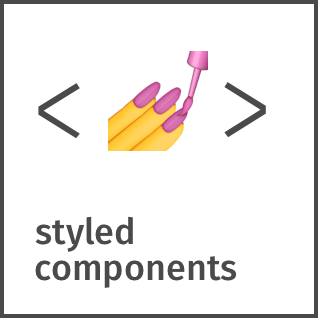
\includegraphics[scale=0.35]{images/hieu/phuluc/styled-components.png}
    \caption{Styled-components}
  \end{center}
\end{figure}
\subsubsection{Ưu điểm}
\begin{itemize}
  \item \textbf{Dễ sử dụng:} Styled-components cung cấp các tính năng và công cụ để tạo và quản lý các kiểu CSS một cách dễ dàng và linh hoạt, giúp tạo ra giao diện người dùng hiện đại và chuyên nghiệp.
  \item \textbf{Tích hợp tốt với React:} Styled-components tích hợp tốt với React, giúp tạo ra các ứng dụng React mạnh mẽ và linh hoạt.
  \item \textbf{Hỗ trợ cho các tính năng CSS:} Styled-components hỗ trợ các tính năng CSS như biến, hàm, và điều kiện, giúp tạo ra các kiểu CSS linh hoạt và dễ bảo trì.
\end{itemize}
\subsubsection{Nhược điểm}
\begin{itemize}
  \item \textbf{Yêu cầu kiến thức về React:} Styled-components yêu cầu kiến thức về React để sử dụng và tùy chỉnh các kiểu CSS, điều này có thể làm tăng độ dốc học đối với người mới sử dụng.
  \item \textbf{Giới hạn về tùy chỉnh:} Styled-components có thể có giới hạn về tùy chỉnh và mở rộng các kiểu CSS so với các thư viện khác.
\end{itemize}
\section{Lập trình Back-end}
\subsection{Kiến thức cơ sở}
\noindent Để thực hiện tốt công việc ở mảng lập trình back-end, chúng ta cần phải có các kiến thức cơ sở, nền
tảng như:
\begin{itemize}
  \item \textbf{Ngôn ngữ lập trình server-side và framework đi kèm:} \\[0.2cm]
  Cần phải vững kiến thức về những ngôn ngữ lập trình như Java, Python, Ruby, PHP, Golang,
  Javascript (Node.js)... Đây là những ngôn ngữ hỗ trợ lập trình phía server, giúp viết các chương
  trình, câu lệnh cho để vận hành ứng dụng, phần mềm, website...\\[0.5cm]
  Ngoài ra, ta cần biết về framework phổ biến đi kèm với mỗi ngôn ngữ để làm việc hiệu quả hơn. Ví
dụ như Java có framework Spring, PHP có Laravel, còn Ruby sẽ là Ruby On Rails...
  \item \textbf{Hệ quản trị cơ sở dữ liệu:}\\[0.2cm]
  Ta cần phải có khả năng quản trị cơ sở dữ liệu theo hệ thống một cách nhanh chóng và quy củ. Để
  làm được điều này, cần nắm rõ cách tổ chức của cơ sở dữ liệu, cấu trúc của cơ sở dữ liệu và các hệ
  thống database như MySQL, Postgres, MongoDB...\\[0.5cm]
  Có hai loại cơ sở dữ liệu là SQL và NoSQL. Cơ sở dữ liệu SQL là cơ sở dữ liệu trong đó dữ liệu
được ánh xạ trong bảng và mỗi cơ sở dữ liệu được liên kết với nhau theo một cách quan trọng, nó
hoạt động trên các truy vấn và tạo ra kết quả dựa trên chúng. Còn đối với NoSQL, nó không giống
như SQL, không cần phải cấu trúc dữ liệu trước, về cơ bản nó hoạt động trên JSON hoặc XML.
  \item \textbf{Kiến thức cơ bản về server (máy chủ):}\\[0.2cm]
  Vì kết quả của việc lập trình back-end sẽ được thực thi trên server nên việc tìm hiểu về server là
  rất cần thiết. Ta cần phải hệ điều hành Linux, một hệ điều hành mã nguồn mở rất nổi tiếng cho
  các máy chủ ngày nay. Bên cạnh đó là kỹ năng để có thể cài đặt các ứng dụng trên server và deploy
  service cũng như các kiến thức về mạng máy tính.\\[0.5cm]
  Một số ví dụ về máy chủ là máy chủ Apache, Nginx, IIS và Microsoft IIS.
  \item \textbf{Kiến thức về API:}\\[0.2cm]
  API là viết tắt của Application Programming Interface, là một phương tiện thông qua đó hai phần
  mềm máy tính có thể giao tiếp với nhau. API là một tập hợp các quy tắc và định nghĩa cho phép
  các ứng dụng khách, phần mềm hoặc dịch vụ khác nhau giao tiếp với nhau qua Internet. Khi hai
  hệ thống giao tiếp, máy chủ là máy cung cấp API và máy khách là người sử dụng nó
\end{itemize}
\subsection{Java}
\subsubsection{Khái niệm}
\noindent Java là một ngôn ngữ lập trình và nền tảng phần mềm có tính "portable" cao, được phát triển bởi Sun Microsystems (nay là Oracle). Nó được thiết kế để chạy trên nhiều hệ điều hành khác nhau thông qua Java Virtual Machine (JVM), và được sử dụng rộng rãi trong phát triển ứng dụng di động, web, và máy tính.\footnote{https://www.java.com/}
\begin{figure}[H]
  \begin{center}
    
\includegraphics[scale=0.3]{images/hieu/phuluc/java.png}
    \caption{Java}
  \end{center}
\end{figure}
\subsubsection{Ưu điểm}
\begin{itemize}
  \item \textbf{Đa năng và linh hoạt:} Java là một ngôn ngữ lập trình đa năng và linh hoạt, được sử dụng rộng rãi trong phát triển ứng dụng web, ứng dụng di động, ứng dụng máy tính, và nhiều lĩnh vực khác.
  \item \textbf{Hiệu suất cao:} Java cung cấp hiệu suất cao và ổn định, giúp phát triển ứng dụng một cách nhanh chóng và hiệu quả.
  \item \textbf{Bảo mật mạnh mẽ:} Java cung cấp các tính năng bảo mật mạnh mẽ như kiểm soát truy cập, mã hóa dữ liệu, và xác thực người dùng, giúp bảo vệ ứng dụng khỏi các mối đe dọa an ninh.
  \item \textbf{Tích hợp tốt với các công nghệ khác:} Java tích hợp tốt với các công nghệ khác như Spring, Hibernate, và Maven, giúp tạo ra các ứng dụng mạnh mẽ và linh hoạt.
  \item \textbf{Hỗ trợ cho các hệ điều hành:} Java hỗ trợ các hệ điều hành phổ biến như Windows, macOS, và Linux, giúp tương thích với nhiều môi trường khác nhau.
\end{itemize}
\subsubsection{Nhược điểm}
\begin{itemize}
  \item \textbf{Yêu cầu kiến thức vững về Java:} Java yêu cầu kiến thức vững về ngôn ngữ lập trình Java để phát triển ứng dụng, điều này có thể làm tăng độ dốc học đối với người mới sử dụng.
  \item \textbf{Cấu hình phức tạp:} Java yêu cầu cấu hình và quản lý ứng dụng một cách cẩn thận, đòi hỏi kiến thức về hệ thống phân tán.
  \item \textbf{Hiệu suất có thể bị ảnh hưởng đối với tải công việc rất cao:} Java có thể gặp vấn đề về hiệu suất đối với tải công việc rất cao, đòi hỏi tối ưu hóa và tinh chỉnh để đạt hiệu suất tốt nhất.
\end{itemize}
\subsection{Framework Java Spring Boot}
\subsubsection{Khái niệm}
\noindent Spring Boot là một framework của Spring Framework, giúp phát triển ứng dụng Java nhanh chóng và dễ dàng thông qua cấu hình tự động và tích hợp sẵn các công cụ quản lý.\footnote{https://spring.io/projects/spring-boot}
\begin{figure}[H]
  \begin{center}
    
\includegraphics[scale=0.3]{images/hieu/phuluc/spring-boot.png}
    \caption{Spring Boot}
  \end{center}
\end{figure}
\subsubsection{Ưu điểm}
\begin{itemize}
  \item \textbf{Dễ sử dụng:} Spring Boot cung cấp các tính năng và công cụ để phát triển ứng dụng một cách nhanh chóng và hiệu quả, giúp tạo ra ứng dụng mạnh mẽ và linh hoạt.
  \item \textbf{Tích hợp tốt với Java:} Spring Boot tích hợp tốt với Java, giúp tạo ra các ứng dụng Java mạnh mẽ và linh hoạt.
  \item \textbf{Hỗ trợ cho các công nghệ khác:} Spring Boot hỗ trợ các công nghệ khác như Hibernate, JPA, và Thymeleaf, giúp tạo ra các ứng dụng mạnh mẽ và linh hoạt.
\end{itemize}
\subsubsection{Nhược điểm}
\begin{itemize}
  \item \textbf{Yêu cầu kiến thức về Java:} Spring Boot yêu cầu kiến thức về Java để sử dụng và tùy chỉnh các ứng dụng, điều này có thể làm tăng độ dốc học đối với người mới sử dụng.
  \item \textbf{Giới hạn về tùy chỉnh:} Spring Boot có thể có giới hạn về tùy chỉnh và mở rộng các ứng dụng so với các framework khác.
\end{itemize}
\subsection{Golang}
\subsubsection{Khái niệm}
\noindent Go (hay còn được gọi là Golang) là một ngôn ngữ lập trình mới, hiện đại, được thiết kế để đơn giản, hiệu quả và dễ dàng để phát triển các hệ thống có hiệu suất cao.\footnote{https://golang.org/}
\begin{figure}[H]
  \begin{center}
    
\includegraphics[scale=0.25]{images/hieu/phuluc/golang.png}
    \caption{Golang}
  \end{center}
\end{figure}
\subsubsection{Ưu điểm}
\begin{itemize}
  \item \textbf{Đa năng và linh hoạt:} Golang là một ngôn ngữ lập trình đa năng và linh hoạt, được sử dụng rộng rãi trong phát triển ứng dụng web, ứng dụng di động, ứng dụng máy tính, và nhiều lĩnh vực khác.
  \item \textbf{Hiệu suất cao:} Golang cung cấp hiệu suất cao và ổn định, giúp phát triển ứng dụng một cách nhanh chóng và hiệu quả.
  \item \textbf{Bảo mật mạnh mẽ:} Golang cung cấp các tính năng bảo mật mạnh mẽ như kiểm soát truy cập, mã hóa dữ liệu, và xác thực người dùng, giúp bảo vệ ứng dụng khỏi các mối đe dọa an ninh.
  \item \textbf{Tích hợp tốt với các công nghệ khác:} Golang tích hợp tốt với các công nghệ khác như Gorilla, Beego, và Revel, giúp tạo ra các ứng dụng mạnh mẽ và linh hoạt.
  \item \textbf{Hỗ trợ cho các hệ điều hành:} Golang hỗ trợ các hệ điều hành phổ biến như Windows, macOS, và Linux, giúp tương thích với nhiều môi trường khác nhau.
\end{itemize}
\subsubsection{Nhược điểm}
\begin{itemize}
  \item \textbf{Yêu cầu kiến thức vững về Golang:} Golang yêu cầu kiến thức vững về ngôn ngữ lập trình Golang để phát triển ứng dụng, điều này có thể làm tăng độ dốc học đối với người mới sử dụng.
  \item \textbf{Cấu hình phức tạp:} Golang yêu cầu cấu hình và quản lý ứng dụng một cách cẩn thận, đòi hỏi kiến thức về hệ thống phân tán.
  \item \textbf{Hiệu suất có thể bị ảnh hưởng đối với tải công việc rất cao:} Golang có thể gặp vấn đề về hiệu suất đối với tải công việc rất cao, đòi hỏi tối ưu hóa và tinh chỉnh để đạt hiệu suất tốt nhất.
\end{itemize}
\subsection{Framework Golang Fiber}
\subsubsection{Khái niệm}
\noindent Fiber là một framework web được xây dựng trên cơ sở ngôn ngữ Go, với mục tiêu tối ưu hóa hiệu suất và sự đơn giản trong việc xây dựng ứng dụng web.\footnote{https://gofiber.io/}
\begin{figure}[H]
  \begin{center}
    
\includegraphics[scale=0.25]{images/hieu/phuluc/fiber.png}
    \caption{Fiber}
  \end{center}
\end{figure}
\subsubsection{Ưu điểm}
\begin{itemize}
  \item \textbf{Dễ sử dụng:} Fiber cung cấp các tính năng và công cụ để phát triển ứng dụng một cách nhanh chóng và hiệu quả, giúp tạo ra ứng dụng mạnh mẽ và linh hoạt.
  \item \textbf{Tích hợp tốt với Golang:} Fiber tích hợp tốt với Golang, giúp tạo ra các ứng dụng Golang mạnh mẽ và linh hoạt.
  \item \textbf{Hỗ trợ cho các công nghệ khác:} Fiber hỗ trợ các công nghệ khác như Gorm, Gqlgen, và Viper, giúp tạo ra các ứng dụng mạnh mẽ và linh hoạt.
  \item \textbf{Hiệu suất cao:} Fiber cung cấp hiệu suất cao và ổn định, giúp phát triển ứng dụng một cách nhanh chóng và hiệu quả.
\end{itemize}
\subsubsection{Nhược điểm}
\begin{itemize}
  \item \textbf{Yêu cầu kiến thức về Golang:} Fiber yêu cầu kiến thức về Golang để sử dụng và tùy chỉnh các ứng dụng, điều này có thể làm tăng độ dốc học đối với người mới sử dụng.
  \item \textbf{Giới hạn về tùy chỉnh:} Fiber có thể có giới hạn về tùy chỉnh và mở rộng các ứng dụng so với các framework khác.
\end{itemize}
\subsection{NodeJS}
\subsubsection{Khái niệm}
\noindent Node.js là một môi trường thực thi mã nguồn mở dựa trên JavaScript, được sử dụng để phát triển ứng dụng web và máy chủ thông qua JavaScript.\footnote{https://nodejs.org/}
\begin{figure}[H]
  \begin{center}
    
\includegraphics[scale=0.3]{images/hieu/phuluc/nodejs.png}
    \caption{Node.js}
  \end{center}
\end{figure}
\subsubsection{Ưu điểm}
\begin{itemize}
  \item \textbf{Đa năng và linh hoạt:} Node.js là một môi trường thực thi mã nguồn mở đa năng và linh hoạt, được sử dụng rộng rãi trong phát triển ứng dụng web, ứng dụng di động, ứng dụng máy tính, và nhiều lĩnh vực khác.
  \item \textbf{Hiệu suất cao:} Node.js cung cấp hiệu suất cao và ổn định, giúp phát triển ứng dụng một cách nhanh chóng và hiệu quả.
  \item \textbf{Bảo mật mạnh mẽ:} Node.js cung cấp các tính năng bảo mật mạnh mẽ như kiểm soát truy cập, mã hóa dữ liệu, và xác thực người dùng, giúp bảo vệ ứng dụng khỏi các mối đe dọa an ninh.
  \item \textbf{Tích hợp tốt với các công nghệ khác:} Node.js tích hợp tốt với các công nghệ khác như Express, Mongoose, và Socket.io, giúp tạo ra các ứng dụng mạnh mẽ và linh hoạt.
  \item \textbf{Hỗ trợ cho các hệ điều hành:} Node.js hỗ trợ các hệ điều hành phổ biến như Windows, macOS, và Linux, giúp tương thích với nhiều môi trường khác nhau.
\end{itemize}
\subsubsection{Nhược điểm}
\begin{itemize}
  \item \textbf{Yêu cầu kiến thức về JavaScript:} Node.js yêu cầu kiến thức về JavaScript để sử dụng và tùy chỉnh các ứng dụng, điều này có thể làm tăng độ dốc học đối với người mới sử dụng.
  \item \textbf{Cấu hình phức tạp:} Node.js yêu cầu cấu hình và quản lý ứng dụng một cách cẩn thận, đòi hỏi kiến thức về hệ thống phân tán.
  \item \textbf{Hiệu suất có thể bị ảnh hưởng đối với tải công việc rất cao:} Node.js có thể gặp vấn đề về hiệu suất đối với tải công việc rất cao, đòi hỏi tối ưu hóa và tinh chỉnh để đạt hiệu suất tốt nhất.
\end{itemize}
\subsection{SocketIO}
\subsubsection{Khái niệm}
\noindent Socket.IO là một thư viện mã nguồn mở dựa trên JavaScript, được sử dụng để tạo và quản lý kết nối thời gian thực giữa máy chủ và máy khách thông qua WebSockets hoặc các giao thức khác.\footnote{https://socket.io/}
\begin{figure}[H]
  \begin{center}
    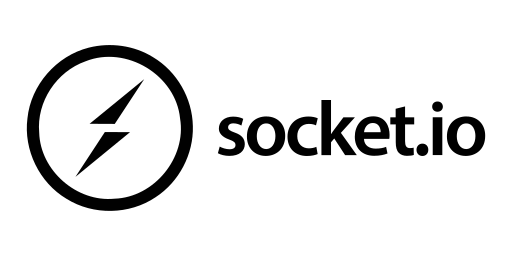
\includegraphics[scale=0.35]{images/hieu/phuluc/socketio.png}
    \caption{Socket.IO}
  \end{center}
\end{figure}
\subsubsection{Ưu điểm}
\begin{itemize}
  \item \textbf{Dễ sử dụng:} Socket.IO cung cấp các tính năng và công cụ để tạo và quản lý kết nối thời gian thực một cách dễ dàng và linh hoạt, giúp tạo ra ứng dụng mạnh mẽ và linh hoạt.
  \item \textbf{Tích hợp tốt với JavaScript:} Socket.IO tích hợp tốt với JavaScript, giúp tạo ra các ứng dụng JavaScript mạnh mẽ và linh hoạt.
  \item \textbf{Hỗ trợ cho các công nghệ khác:} Socket.IO hỗ trợ các công nghệ khác như Node.js, React, và Angular, giúp tạo ra các ứng dụng mạnh mẽ và linh hoạt.
\end{itemize}
\subsubsection{Nhược điểm}
\begin{itemize}
  \item \textbf{Yêu cầu kiến thức về JavaScript:} Socket.IO yêu cầu kiến thức về JavaScript để sử dụng và tùy chỉnh các kết nối thời gian thực, điều này có thể làm tăng độ dốc học đối với người mới sử dụng.
  \item \textbf{Giới hạn về tùy chỉnh:} Socket.IO có thể có giới hạn về tùy chỉnh và mở rộng các kết nối thời gian thực so với các thư viện khác.
\end{itemize}
\subsection{PostgreSQL}
\subsubsection{Khái niệm}
\noindent PostgreSQL là một hệ quản trị cơ sở dữ liệu mã nguồn mở dựa trên SQL, được sử dụng để lưu trữ và quản lý dữ liệu trong ứng dụng web và máy chủ.\footnote{https://www.postgresql.org/}
\begin{figure}[H]
  \begin{center}
    
\includegraphics[scale=0.3]{images/hieu/phuluc/postgresql.png}
    \caption{PostgreSQL}
  \end{center}
\end{figure}
\subsubsection{Ưu điểm}
\begin{itemize}
  \item \textbf{Đa năng và linh hoạt:} PostgreSQL là một hệ quản trị cơ sở dữ liệu đa năng và linh hoạt, được sử dụng rộng rãi trong phát triển ứng dụng web, ứng dụng di động, ứng dụng máy tính, và nhiều lĩnh vực khác.
  \item \textbf{Hiệu suất cao:} PostgreSQL cung cấp hiệu suất cao và ổn định, giúp lưu trữ và quản lý dữ liệu một cách nhanh chóng và hiệu quả.
  \item \textbf{Bảo mật mạnh mẽ:} PostgreSQL cung cấp các tính năng bảo mật mạnh mẽ như kiểm soát truy cập, mã hóa dữ liệu, và xác thực người dùng, giúp bảo vệ dữ liệu khỏi các mối đe dọa an ninh.
  \item \textbf{Tích hợp tốt với các công nghệ khác:} PostgreSQL tích hợp tốt với các công nghệ khác như Node.js, Django, và Ruby on Rails, giúp tạo ra các ứng dụng mạnh mẽ và linh hoạt.
  \item \textbf{Hỗ trợ cho các hệ điều hành:} PostgreSQL hỗ trợ các hệ điều hành phổ biến như Windows, macOS, và Linux, giúp tương thích với nhiều môi trường khác nhau.
\end{itemize}
\subsubsection{Nhược điểm}
\begin{itemize}
  \item \textbf{Yêu cầu kiến thức về SQL:} PostgreSQL yêu cầu kiến thức về SQL để sử dụng và quản lý cơ sở dữ liệu, điều này có thể làm tăng độ dốc học đối với người mới sử dụng.
  \item \textbf{Cấu hình phức tạp:} PostgreSQL yêu cầu cấu hình và quản lý cơ sở dữ liệu một cách cẩn thận, đòi hỏi kiến thức về hệ thống phân tán.
  \item \textbf{Hiệu suất có thể bị ảnh hưởng đối với tải công việc rất cao:} PostgreSQL có thể gặp vấn đề về hiệu suất đối với tải công việc rất cao, đòi hỏi tối ưu hóa và tinh chỉnh để đạt hiệu suất tốt nhất.
\end{itemize}
\section{Triển khai hệ thống}
\subsection{Docker}
\subsubsection{Khái niệm}
\noindent Docker là một nền tảng mã nguồn mở dựa trên Linux, được sử dụng để triển khai và quản lý các ứng dụng trong môi trường container, giúp tạo ra các ứng dụng mạnh mẽ và linh hoạt.\footnote{https://www.docker.com/}
\begin{figure}[H]
  \begin{center}
    
\includegraphics[scale=0.35]{images/hieu/phuluc/docker.png}
    \caption{Docker}
  \end{center}
\end{figure}
\subsubsection{Ưu điểm}
\begin{itemize}
  \item \textbf{Dễ sử dụng:} Docker cung cấp các tính năng và công cụ để triển khai và quản lý ứng dụng một cách dễ dàng và linh hoạt, giúp tạo ra ứng dụng mạnh mẽ và linh hoạt.
  \item \textbf{Tích hợp tốt với Linux:} Docker tích hợp tốt với Linux, giúp tạo ra các ứng dụng Linux mạnh mẽ và linh hoạt.
  \item \textbf{Hỗ trợ cho các công nghệ khác:} Docker hỗ trợ các công nghệ khác như Kubernetes, Jenkins, và Prometheus, giúp tạo ra các ứng dụng mạnh mẽ và linh hoạt.
  \item \textbf{Hiệu suất cao:} Docker cung cấp hiệu suất cao và ổn định, giúp triển khai ứng dụng một cách nhanh chóng và hiệu quả.
\end{itemize}
\subsubsection{Nhược điểm}
\begin{itemize}
  \item \textbf{Yêu cầu kiến thức về Linux:} Docker yêu cầu kiến thức về Linux để triển khai và quản lý ứng dụng, điều này có thể làm tăng độ dốc học đối với người mới sử dụng.
  \item \textbf{Cấu hình phức tạp:} Docker yêu cầu cấu hình và quản lý ứng dụng một cách cẩn thận, đòi hỏi kiến thức về hệ thống phân tán.
  \item \textbf{Hiệu suất có thể bị ảnh hưởng đối với tải công việc rất cao:} Docker có thể gặp vấn đề về hiệu suất đối với tải công việc rất cao, đòi hỏi tối ưu hóa và tinh chỉnh để đạt hiệu suất tốt nhất.
\end{itemize}
\subsection{Kubernetes}
\subsubsection{Khái niệm}
\noindent Kubernetes là một nền tảng mã nguồn mở dựa trên Linux, được sử dụng để triển khai và quản lý các ứng dụng trong môi trường container, giúp tạo ra các ứng dụng mạnh mẽ và linh hoạt.\footnote{https://kubernetes.io/}
\begin{figure}[H]
  \begin{center}
    
\includegraphics[scale=0.3]{images/hieu/phuluc/kubernetes.png}
    \caption{Kubernetes}
  \end{center}
\end{figure}
\noindent Các ứng dụng có sử dụng Kubernetes: Google, Netflix, Airbnb, Spotify, Grab, Zalando, Adidas...và nhiều hơn nữa. Kubernetes đã trở thành một công nghệ phổ biến và mạnh mẽ trong việc quản lý và triển khai ứng dụng quy mô lớn.
\subsubsection{Kiến trúc}
\noindent Hình ảnh được tham khảo từ bài viết "What Is Kubernetes Architecture? - Components Overview"\footnote{https://spacelift.io/blog/kubernetes-architecture}
 \begin{figure}[H]
    \begin{center}
    \includegraphics[scale = 0.2]{images/phat/kubernetes_architecture.jpg}
    \vspace*{7mm}
    \caption{Kubernetes Architecture }
    \end{center}
    \label{}
\end{figure}
\noindent Kiến trúc của Kubernetes bao gồm:
\begin{itemize}
    \item Master Node: Quản lý, điều phối và giám sát toàn bộ hệ thống Kubernetes.
    \item Worker Node: Chứa các container và chịu trách nhiệm thực hiện các tác vụ đồng bộ từ Master Node.
    \item Pod: Nhóm các container chạy cùng nhau trên cùng một Worker Node, chia sẻ tài nguyên và mạng.
    \item Service: Một tập hợp các Pod có thể truy cập thành một đầu nối duy nhất từ bên ngoài.
    \item Volume: Cung cấp quản lý lưu trữ cho các container trong Pod.
\end{itemize}
\subsubsection{Cách thiết lập Kubernetes cho ứng dụng}
\begin{itemize}
    \item Định nghĩa và triển khai mô tả ứng dụng: Sử dụng các tệp cấu hình (ví dụ: YAML) để định nghĩa ứng dụng, bao gồm Pod, Service và các tài nguyên khác.
    \item Triển khai và quản lý: Gửi yêu cầu triển khai tới Master Node, sau đó Kubernetes sẽ triển khai các Pod và Service, quản lý vòng đời và giám sát.
    \item Tự động mở rộng và cân bằng tải: Kubernetes tự động mở rộng hoặc thu hẹp quy mô của các Pod để đáp ứng tải công việc và cân bằng tải giữa các Worker Node.
\end{itemize}
\subsubsection{Ưu điểm}
\begin{itemize}
  \item \textbf{Tính mở rộng:} Kubernetes có khả năng mở rộng dễ dàng, cho phép triển khai và quản lý các ứng dụng có quy mô lớn mà không gặp vấn đề về hiệu suất.
  \item \textbf{Tự động hoá:} Kubernetes cung cấp các công cụ tự động hóa việc triển khai, mở rộng và quản lý ứng dụng, giúp giảm thiểu công sức và thời gian mà nhà quản trị hệ thống cần phải bỏ ra.
  \item \textbf{Tính đa nền tảng:} Kubernetes có thể hoạt động trên nhiều loại môi trường, từ on-premise đến cloud public và private, tạo điều kiện thuận lợi cho việc di động giữa các môi trường.
  \item \textbf{Tính ổn định và độ tin cậy cao:} Kubernetes đã được sử dụng rộng rãi trong các môi trường sản xuất và được cộng đồng hỗ trợ mạnh mẽ, giúp tăng tính ổn định và tin cậy của nền tảng.
  \item \textbf{Tính linh hoạt và tuỳ biến:} Kubernetes cho phép người dùng tuỳ chỉnh và cấu hình theo nhu cầu của từng ứng dụng hoặc môi trường cụ thể.
  \item \textbf{Tính dễ mở rộng và mạnh mẽ:} Kubernetes tích hợp nhiều tính năng như service discovery, load balancing, self-healing, và auto-scaling, giúp tạo ra môi trường chạy ứng dụng linh hoạt và mạnh mẽ.
\end{itemize}
\subsubsection{Nhược điểm}
\begin{itemize}
  \item \textbf{Yêu cầu kiến thức vững về Linux:} Kubernetes yêu cầu kiến thức vững về Linux để triển khai và quản lý ứng dụng, điều này có thể làm tăng độ dốc học đối với người mới sử dụng.
  \item \textbf{Phức tạp trong triển khai ban đầu:} Kubernetes yêu cầu một khối lượng kiến thức lớn và thời gian đầu tư lớn để triển khai và quản lý hiệu quả. Việc cấu hình và triển khai một cluster Kubernetes có thể khó khăn đối với những người mới bắt đầu.
  \item \textbf{Yêu cầu tài nguyên cao:} Kubernetes cần một tài nguyên phần cứng và mạng đáng kể để hoạt động hiệu quả. Điều này có thể là một thách thức đối với các tổ chức có ngân sách hạn chế hoặc không có sẵn cơ sở hạ tầng mạng và lưu trữ phù hợp.
\end{itemize}
\subsection{Minikube}
\subsubsection{Khái niệm}
\noindent Minikube là một công cụ mã nguồn mở dựa trên Linux, được sử dụng để triển khai và quản lý một cluster Kubernetes trên máy tính cá nhân hoặc máy chủ, giúp tạo ra môi trường phát triển và thử nghiệm ứng dụng mạnh mẽ và linh hoạt.\footnote{https://minikube.sigs.k8s.io/}
\begin{figure}[H]
  \begin{center}
    
\includegraphics[scale=0.35]{images/hieu/phuluc/minikube.png}
    \caption{Minikube}
  \end{center}
\end{figure}
\subsubsection{Ưu điểm}
\begin{itemize}
  \item \textbf{Dễ cài đặt và sử dụng} Minikube cung cấp một cách đơn giản để cài đặt một cluster Kubernetes trên máy tính cá nhân chỉ trong vài bước đơn giản, giúp nhà phát triển nhanh chóng bắt đầu làm việc với Kubernetes.
  \item \textbf{Tính di động và độc lập:} Với Minikube, bạn có thể tạo và chạy một cluster Kubernetes độc lập trên máy tính của mình mà không cần phụ thuộc vào cơ sở hạ tầng mạng hoặc máy chủ ngoài.
  \item \textbf{Giả lập môi trường sản xuất:} Minikube cung cấp một cách để tạo ra một môi trường giả lập tương tự như môi trường sản xuất, giúp nhà phát triển kiểm tra và thử nghiệm ứng dụng của họ trước khi triển khai vào môi trường thực tế.
  \item \textbf{Hỗ trợ nhiều môi trường:} Minikube có thể chạy trên nhiều hệ điều hành như Linux, macOS và Windows, giúp đáp ứng nhu cầu phát triển trên nhiều nền tảng khác nhau.
  \item \textbf{Tính linh hoạt và tuỳ chỉnh:} Minikube cho phép bạn tùy chỉnh cấu hình của cluster Kubernetes tạo ra, bao gồm số lượng node, tài nguyên hệ thống, và các tính năng khác.
\end{itemize} 
\subsubsection{Nhược điểm}
\begin{itemize}
  \item \textbf{Giới hạn về quy mô:} Minikube có giới hạn về quy mô của cluster Kubernetes mà bạn có thể tạo ra, điều này có thể gây khó khăn đối với việc thử nghiệm và phát triển ứng dụng có quy mô lớn.
  \item \textbf{Yêu cầu tài nguyên hệ thống:} Minikube cần một số tài nguyên hệ thống đáng kể để hoạt động hiệu quả, điều này có thể là một thách thức đối với các máy tính cá nhân có cấu hình yếu hoặc không đáp ứng được yêu cầu tài nguyên.
  \item \textbf{Yêu cầu kiến thức về Kubernetes:} Minikube yêu cầu kiến thức về Kubernetes để triển khai và quản lý cluster, điều này có thể làm tăng độ dốc học đối với người mới sử dụng.
\end{itemize}
\subsection{RabbitMQ}
\subsubsection{Khái niệm}
\noindent RabbitMQ là một hệ thống message broker mã nguồn mở, được sử dụng để truyền thông giữa các ứng dụng và dịch vụ thông qua các message queue, giúp tạo ra các ứng dụng mạnh mẽ và linh hoạt.\footnote{https://www.rabbitmq.com/}
\begin{figure}[H]
  \begin{center}
    
\includegraphics[scale=0.3]{images/hieu/phuluc/rabbitmq.png}
    \caption{RabbitMQ}
  \end{center}
\end{figure}

\subsubsection{Kiến trúc của RabbitMQ}
\begin{itemize}
    \item Producer:

Là thành phần tạo ra và gửi các thông điệp (message).
Message được gửi đến một exchange.
    \item Exchange:

Nhận thông điệp từ nhà sản xuất và định tuyến chúng đến hàng đợi (queue) thích hợp.
Có các loại định tuyến khác nhau như direct, topic, fanout, và headers, cho phép định tuyến dựa trên các tiêu chí khác nhau.
    \item Queue (Hàng đợi):

Là nơi lưu trữ các thông điệp đến từ sàn giao dịch cho đến khi chúng được xử lý bởi một tiêu thụ (consumer).
Các hàng đợi có thể được chia sẻ giữa nhiều tiêu thụ hoặc có thể chỉ được sử dụng bởi một tiêu thụ cụ thể.
    \item Binding (Ràng buộc):

Liên kết giữa một exchange và một queue, xác định cách thông điệp nên được định tuyến từ exchange đến queue.
Ràng buộc này được thiết lập thông qua các quy tắc định tuyến (routing key).
    \item Consumer:

Là thành phần đọc và xử lý các thông điệp từ hàng đợi.
Có thể có nhiều tiêu thụ cùng một lúc đọc từ cùng một hàng đợi.
    \item Virtual Host:

Là một không gian làm việc ảo trong RabbitMQ, giúp tách biệt và cô lập các ứng dụng và người dùng khác nhau.
Mỗi Virtual Host có thể có các exchange, queue, và quyền riêng biệt.
    \item Broker:

Là nền tảng hoạt động của RabbitMQ.
Nhận thông điệp từ nhà sản xuất, định tuyến chúng đến hàng đợi thông qua sàn giao dịch và chuyển giao chúng đến các tiêu thụ.
    \item Connection:

Là một kết nối mạng giữa ứng dụng và RabbitMQ Broker.
Mỗi ứng dụng có thể có nhiều kết nối.
\end{itemize}
\begin{figure}[H]

    \begin{center}
    \includegraphics[scale = 0.5]{images/phat/rabbitMQ.png}
    \vspace*{7mm}
    \caption{RabbitMQ Architecture}
    \end{center}
    \label{}
\end{figure}
\subsubsection{Ưu điểm}
\begin{itemize}
  \item \textbf{Tính tin cậy cao:} RabbitMQ được thiết kế để đảm bảo tin cậy trong việc giao tiếp và xử lý thông điệp. Nó hỗ trợ nhiều phương thức xác nhận và bảo đảm việc không mất thông điệp.
  \item \textbf{Khả năng mở rộng tốt:} RabbitMQ có thể mở rộng để đáp ứng nhu cầu của các ứng dụng với lượng lớn thông điệp thông qua các cơ chế như clustering và phân phối tải
  \item \textbf{Tính linh hoạt:} RabbitMQ hỗ trợ nhiều giao thức như AMQP, MQTT, STOMP, giúp tương thích với nhiều loại ứng dụng và tình huống sử dụng khác nhau.
  \item \textbf{Quản lý linh hoạt:} RabbitMQ cung cấp các công cụ quản lý mạnh mẽ, cho phép quản trị viên giám sát và điều chỉnh hệ thống một cách dễ dàng.
\end{itemize}
\subsubsection{Nhược điểm}
\begin{itemize}
  \item \textbf{Phức tạp trong triển khai:} Cài đặt và cấu hình RabbitMQ có thể phức tạp đối với những người mới bắt đầu, đặc biệt là trong một môi trường phức tạp.
  \item \textbf{Yêu cầu tài nguyên cao:} RabbitMQ có thể đòi hỏi một lượng lớn tài nguyên hệ thống, đặc biệt là bộ nhớ, để xử lý và lưu trữ thông điệp.
  \item \textbf{Độ trễ định tuyến:} Trong một số trường hợp, RabbitMQ có thể gây ra độ trễ định tuyến khi xử lý các thông điệp, đặc biệt là trong các mô hình phân tán lớn.
\end{itemize}